\section{2004 - PHYSICS 2A ALTERNATIVE A PRACTICAL}

\begin{enumerate}
\item[1.] The aim of this experiment is to determine the mass of a given dry cell, size ``AA''.\\[5pt]

You are provided with a dry cell, a knife edge, two weights 50 g and 20 g, and a metre rule.\\[5pt]

Proceed as follows:
\begin{enumerate}
\item[(a)] Locate and note the centre of gravity C of the metre rule by balancing on the knife edge.
\item[(b)] Suspend the 50 g mass on one side of the metre rule, and 20 g together with the dry cell on the other side of the metre rule adjusting their position until the metre rule balances horizontally, as shown in Figure 1 below.

\begin{center}
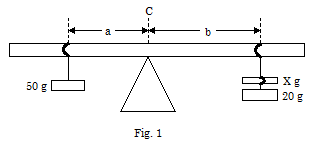
\includegraphics[width=10cm]{./img/2004-1-alt.png}
\end{center}

\item[(c)] By fixing a = 5 cm from C find its corresponding length, b, from C.
\item[(d)] Repeat and tabulate your results using a = 10 cm, 15 cm, 20 cm and 25 cm.
\item[(e)] Draw a graph of ``a'' against ``b'' and calculate its slope G.
\item[(f)] Calculate X from the equation $\text{G} = \cfrac{20 + \text{X}}{50}$. \hfill \textbf{(25 marks)}
\end{enumerate}


\item[2.] You are provided with a glass block, drawing board, optical pins and plane papers.\\

Place a white piece of paper on the drawing board. Place the glass block with one of its largest surface top most on top of the white paper. Mark the outline of the glass block on the paper with a pencil. Remove the glass block and draw a normal as shown in Figure 2 below.

\begin{center}
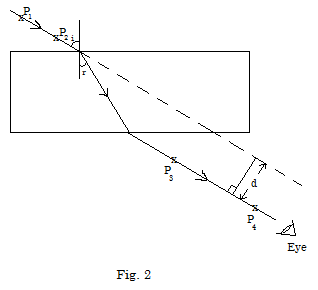
\includegraphics[width=10cm]{./img/2004-2-alt.png}
\end{center}

\begin{enumerate}
\item[(a)] Draw a line making an angle of incidence, $i$ of $30^\circ$. Erect two pins P$_1$ and P$_2$ on this line at a suitable distance apart. Replace the glass block and erect two more pins P$_3$ and P$_4$ at positions which appear to be in a straight line with the other two pins as seen through the glass block from the other side.\\[10pt]

Remove the glass block and draw the complete path of the ray (see Fig. 2). Measure the angle of refraction, $r$.
\item[(b)]
\begin{enumerate}
\item[(i)] Extend the direction of the incident ray as shown by the dotted line.
\item[(ii)] Measure the perpendicular distance `$d$' between extended incident ray and the emergent ray.
\end{enumerate}
\item[(c)] Repeat the procedure in (a) and (b) above for angles of incidence of $30^\circ$, $40^\circ$, $50^\circ$, $60^\circ$ and $70^\circ$. (In each case make your drawings on a fresh part of the drawing paper).
\item[(d)] Tabulate your results as shown in Table 1 below.
\begin{center}
\begin{tabular}{|p{0.15\textwidth}|p{0.15\textwidth}|p{0.15\textwidth}|p{0.15\textwidth}|p{0.15\textwidth}|} \hline
\multicolumn{1}{|c|}{$i$ (deg)} & \multicolumn{1}{c|}{$r$ (deg)} & \multicolumn{1}{c|}{$d$ (cm)} & \multicolumn{1}{c|}{$d\cos{r}$} & \multicolumn{1}{c|}{$\sin{(i-r)}$} \\ \hline
\multicolumn{1}{|c|}{30}&&&& \\
\multicolumn{1}{|c|}{40}&&&& \\
\multicolumn{1}{|c|}{50}&&&& \\
\multicolumn{1}{|c|}{60}&&&& \\
\multicolumn{1}{|c|}{70}&&&& \\ \hline
\end{tabular}\\[10pt]
\end{center}
\begin{enumerate}
\item[(i)] Plot a graph of $d\cos{r}$ against $\sin{(i-r)}$.
\item[(ii)] Find the gradient of the graph.
\item[(iii)] Measure the width of the glass block.
\item[(iv)] How is the gradient of the graph in 2 (a)(ii) and the width of the glass block in 2 (a)(iii) related?\\[5pt]
\end{enumerate}
\item[] NB: \quad Hand in your diagrams (drawings) together with your answer booklet. 
\item[] \flushright \textbf{(25 marks)}

\end{enumerate}

\item[3.] Determine the resistivity $\rho$ of the wire labelled W and the internal resistance of the battery provided.\\

Proceed as follows:

\begin{center}
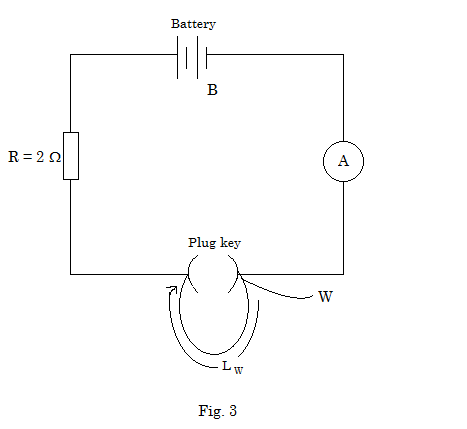
\includegraphics[width=10cm]{./img/2004-3-alt.png}
\end{center}

Connect the circuit as shown in fig. 3 above. With the plug key open adjust the length of wire W to a value of 20 cm. Note the ammeter reading.\\[10pt]

\noindent NB: The plug key should remain open throughout the experiment.

\begin{enumerate}
\item[(a)] Repeat the procedure above for $L_W$ = 40 cm, 60 cm, 80 cm and 100 cm each time recording the ammeter reading.
\item[(b)] Tabulate your results as shown in Table 2 below.

\begin{tabular}{|p{2.5cm}|c|c|} \hline
Length $L_W$ of wire (cm)& Current $I$ (A)& $\cfrac{1}{I} \left(\text{A}^{-1}\right)$ \\ \hline
&& \\
&& \\
&& \\
&& \\ \hline
\end{tabular}\\[10pt]

\item[(c)]
\begin{enumerate}
\item[(i)] Plot a graph of $\cfrac{1}{I}$ (vertical) against $L_W$ (horizontal).
\item[(ii)] Determine the slope G.
\item[(iii)] Determine the intercept $Y$ on the vertical axis.
\end{enumerate}
\item[(d)] Measure and record the diameter at four different places on the wire. Hence find the mean value of diameter $d$.
\item[(e)] Given that $G = \cfrac{4\rho}{\pi d^2E}$ and $Y = \cfrac{R + r}{E}$\\[10pt]
Where $E$ is the emf of the battery, and $R = 2 \Omega$, Find the
\begin{enumerate}
\item[(i)] Resistivity $\rho$ of the wire.
\item[(ii)]	Internal resistance $r$ of the battery. \hfill \textbf{(25 marks)}
\end{enumerate}
\end{enumerate}

\end{enumerate}